\documentclass[11pt,letterpaper]{article}

\usepackage[english]{babel}
\usepackage[utf8]{inputenc}

\usepackage{amsmath}
\usepackage{amssymb}
\usepackage{graphicx}

\usepackage[top=1in, bottom=1in, left=1in, right=1in]{geometry}
\graphicspath{{./imagenes/}}

\begin{document}
	
	\begin{titlepage}
		\centering
		
		{\scshape\LARGE Universidad Nacional Autónoma de México \par}
		
		\vspace{1cm}
		{\scshape\Large Facultad de Ciencias\par}
		\vspace{1.5cm}
		
		\begin{figure}[h]
			\centering
			
\includegraphics[scale=0.15]{logo.png}
		\end{figure}
		
		\vspace{.8 cm}
		
		{\LARGE Práctica 04 \par}
		
		\vspace{0.5cm}
		\large{\itshape{Vianey Aileen Borrás Pablo}} \small{ - 316033619} \\ \vspace{0.3cm}
		\large{\itshape{Kevin Axel Prestegui Ramos}} \small{ - 316201373} \\ \vspace{0.3cm}
		\vfill
		
		\textbf{Arquitectura de Computadoras}\\
		\textbf{Dr. Jorge Luis Ortega Arjona}. \par
		\vspace{0.5cm}
		Fecha de entrega: \textbf{12 de marzo de 2020}.
	\end{titlepage}

	\textbf{PREGUNTAS}
		\begin{itemize}
			\item Crea un decodificador de 3x8 usando decodificadores 2x4.
			
			Para poder crearlo, necesitamos primero saber su tabla de verdad 
			\begin{figure}[h!]
				\centering
				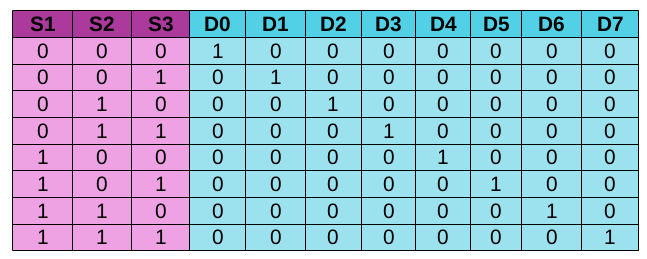
\includegraphics[scale=0.5]{3x8.png}
				\caption{Tabla de verdad de un codificador de 3x8}
			\end{figure}
			
			Si analizamos la tabla de verdad de un codificador de 3x8 y la dividimos en dos partes una donde S1=0 y otra donde S2=1 obtenemos las siguientes tablas.
			
			$\bullet$ Cuando S1=0:\\
			Observemos en la tabla donde S1=0, cuando de D0 hasta D3 están activadas se comportan igual que el decodificador de 2x4.
			
			$\bullet$ Cuando S1=1:\\
			Ahora observemos que cuando S1=1 y las señales de D4 hasta D7 están activadas se comportan igual que el decodificador de 2x4.			
			
			\begin{figure}[h!]
				\centering
				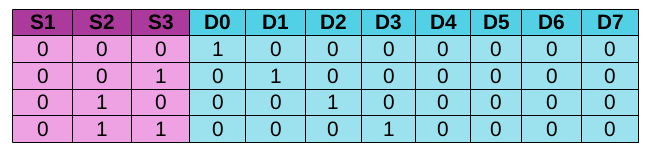
\includegraphics[scale=0.35]{uno.png}				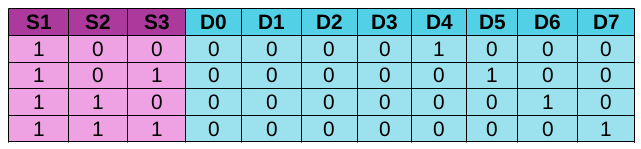
\includegraphics[scale=0.35]{dos.png}
				
			\end{figure}
			
			Por lo tanto para crear el decodificador de 3x8 necesitamos usar dos decodificadores de 2x4.Recordemos que el circuito de un decodificador de 2x4 se ve de la siguiente manera:
			
			\begin{figure}[h!]
				\centering
				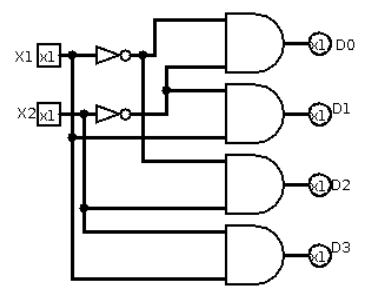
\includegraphics[scale=0.5]{deco.png}
			\end{figure}
			
			
			\newpage
			\item Crea un enunciado parecido a los de las prácticas anteriores (Club de	Toby) y crea dos circuitos que lo resuelvan, uno utilizando un decodificador y el otro sin decodificador (No es necesario que minimicen, pero puedes hacerlo).\\
			
			El club de Toby tiene 4 integrantes, el cuál se rige por votos para tomar sus decisiones, el cumpleaños de Toby se acerca y los otros tres integrantes planean hacerle una fiesta sorpresa, por lo que los integrantes deciden votar para ver si se realiza o no, recordemos que el voto de Toby cuenta doble, mientras que los otros solo tienen derecho a votar una sola vez.
			
			\begin{figure}[h!]
				\centering
				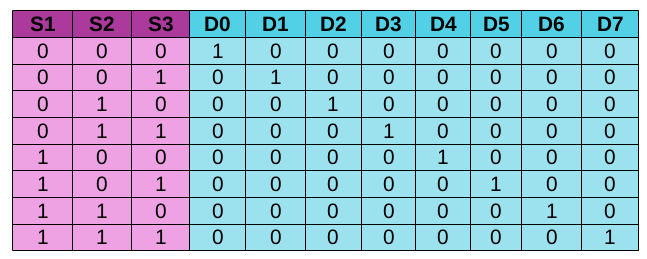
\includegraphics[scale=0.5]{3x8.png}
				\caption{Tabla del Decodificador}
				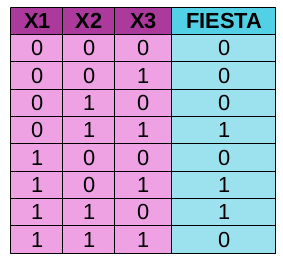
\includegraphics[scale=0.5]{fiesta.png}
				\caption{Tabla de verdad}
			\end{figure}
			
			\newpage
			
			\item ¿Cómo implementarías un decodificador de 4x16 usando únicamente decodificadores de 2x4?, ¿Cuántos de estos (2x4) necesitarías?
			
			Sabemos que un decodificador de 4x16 tiene 4 entradas y 16 salidas y su tabla de verdad se ve como sigue:
			
			\begin{figure}[h!]
				\centering
				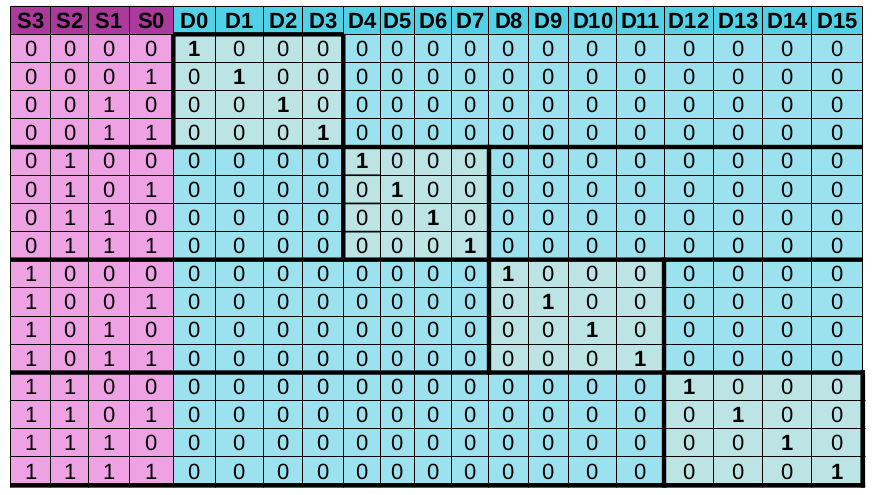
\includegraphics[scale=0.4]{3.png}
			\end{figure}
			
			Observemos que si la tabla la dividimos en bloque de 4 obtenemos cuatro casos donde:
			
			$\bullet$ Cuando S$_3$=0 y S$_2$=0\\
			De D$_0$ hasta D$_3$ están activadas, entonces se comportan igual que el decodificador de 2x4.
			
			$\bullet$ Cuando S$_3$=0 y S$_2$=1\\
			De D$_4$ hasta D$_7$ están activadas, entonces se comportan igual que el decodificador de 2x4.
			
			$\bullet$ Cuando S$_3$=1 y S$_2$=0\\
			De D$_8$ hasta D$_11$ están activadas, entonces se comportan igual que el decodificador de 2x4.
			
			$\bullet$ Cuando S$_3$=1 y S$_2$=1\\
			De D$_12$ hasta D$_15$ están activadas, entonces se comportan igual que el decodificador de 2x4.	
			
			Basándonos en lo anterior necesitamos 4 decodificadores de 2x4 para las 16 salidas, pero necesitamos otro decodificador el cual se encargue de habilitar cado uno de los cuatro decodificadores.
			
			\begin{figure}[h!]
				\centering
				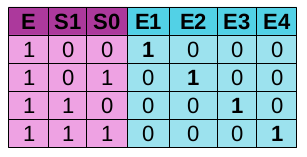
\includegraphics[scale=0.4]{4.png}
			\end{figure}
		
		Por lo tanto necesitamos 5 decodificadores de 2x4\\
			
		\end{itemize}

\end{document}